%!TEX root = usersmanual.tex
\chapter{\textsc{Appendix}}

	\section{Externally Specified Parameters}
		\subsection*{txtl\_reaction\_config (class)}
		The txtl\_reaction\_config class enables users to input custom reaction parameters for the TXTL extract into their model. This is done via a comma-separated-value (.csv) file. The parameters controlled by this class are given in the properties of this class. 
		\subsubsection*{List of Parameters}
			\begin{enumerate}
			\item \textsc{NTPmodel}: 
			There are two models for transcription that the toolbox can switch between, model 1 and 2. We recommend keeping this setting at model 2, since model 1 suffers from stiffness of the differential equations to be solved, and is primarily used for testing purposes. 
        	\item \textsc{AAmodel}: 
        	Similar to NTPmodel above, we recommend keeping this setting at 2. 
        	\item \textsc{Transcription\_Rate}:
        	
        	\begin{align}
        	& \mathrm{NTP:RNAP^{70}:DNA} \rightarrow \mathrm{DNA} + \mathrm{RNA} + \mathrm{RNAP} \\
        	\end{align}
        	This is the reaction for transcription, with transcription rate calculated as:\\
        	\begin{align}
        	& \textsc{Transcription\_Rate} = \frac{(log(2)\times50)}{RNA\_length}\\
        	\end{align}
        	\textrm{and a dummy reaction for NTP consumption, with rate \textsc{Transcription\_Rate\_dummy}} \\
        	\begin{align}
        	& \mathrm{NTP:RNAP^{70}:DNA} \rightarrow \mathrm{DNA} + \mathrm{RNAP} \\ 
        	& \textsc{Transcription\_Rate\_dummy} = \left(\frac{RNA\_length}{100}-1\right)\times\textsc{Transcription\_Rate}
        	\end{align}
        	
        	\item \textsc{Translation\_Rate}: Reaction rate for: \\
        	% '[AA:' Ribobound.Name '] -> ' rna.Name ' + ' protein.Name ' +  Ribo'
        	\begin{align}
        	& \mathrm{ATP:AA:Ribo:RNA}  \rightarrow \mathrm{Protein} + \mathrm{RNA} + \mathrm{Ribo}\\
        	\end{align}
        	This is the reaction for translation, with reaction rate calculated as:\\
        	\begin{align}
        	& \textsc{Translation\_Rate} = \frac{(log(2)\times0.64)}{protein\_length}\\
        	\end{align}
        	\textrm{and a dummy reaction for AA consumption, with rate \textsc{Translation\_Rate\_dummy}} \\
        	\begin{align}
        	&\mathrm{ATP:AA:Ribo:RNA}  \rightarrow \mathrm{RNA} + \mathrm{Ribo} + \mathrm{ATP}\\
        	& \textsc{Translation\_Rate\_dummy} = \left(\frac{protien\_length}{100}-1\right)\times\textsc{Translation\_Rate}
        	\end{align}
        	
        	\item \textsc{DNA\_RecBCD\_Forward and DNA\_RecBCD\_Reverse}:
        	Complex formation and dissociation rate between RecBCD enzyme and DNA.        	
        	\begin{align}
        	& \mathrm{DNA} + \mathrm{RecBCD}  \rightleftharpoons \mathrm{DNA:RecBCD}
        	\end{align}
        	
        	
        	\item \textsc{DNA\_RecBCD\_complex\_deg}: 
        	Degradation rate of RecBCD-DNA complex. 
        	\begin{align}
        	& \mathrm{DNA:RecBCD} \rightarrow  \mathrm{RecBCD} 
        	\end{align}
        	
        	\item \textsc{Protein\_ClpXP\_Forward and Protein\_ClpXP\_Reverse}: 
        	
        	Complex formation and dissociation rate between ClpXP enzyme and a protein tagged for degradation.
        	\begin{align}
        	& \mathrm{Protein} + \mathrm{ClpXP} \rightleftharpoons  \mathrm{Protein:ClpXP} 
        	\end{align}        	
        	\item \textsc{Protein\_ClpXP\_complex\_deg} 
        	Degradation rate of ClpXP-Protein complex.
        	\begin{align}
        	& \mathrm{Protein:ClpXP}  \rightarrow   \mathrm{ClpXP}
        	\end{align} 
        	\item \textsc{RNAP\_S70\_F and RNAP\_S70\_R}:
        	RNAP70 formation and dissociation rate.
        	\begin{align}
        	& \mathrm{RNAP} + \sigma^{70} \rightleftharpoons   \mathrm{RNAP^{70}}
        	\end{align}
        	\item \textsc{AA\_Forward and AA\_Reverse}:
        	Binding and dissociation of AA to Ribosome mRNA complex:
        	\begin{align}
        	& \mathrm{AA} + \mathrm{Ribo:RNA}  \rightleftharpoons   \mathrm{AA}:\mathrm{Ribo:RNA}
        	\end{align}
        	\item \textsc{Ribosome\_Binding\_F and Ribosome\_Binding\_R}: Binding and dissociation rated fro RNA-Ribosome complex:
        	\begin{align}
        	& \mathrm{Ribo} + \mathrm{RNA}  \rightleftharpoons   \mathrm{Ribo:RNA}
        	\end{align}
        	\item \textsc{RNA\_deg}: RNA degradation rate:
        	\begin{align}
        	& \mathrm{RNA} + \mathrm{RNAase}  \rightarrow   \mathrm{RNAase}
        	\end{align}
        	
        	\item \textsc{NTP\_Forward and NTP\_Reverse}:
        	Binding and dissociation of NTP to the RNAP70-DNA complex:
        	% [' RNAPbound '] + NTP <-> [NTP:' RNAPbound ']
        	\begin{align}
        	& \mathrm{NTP} + \mathrm{RNAP^{70}}:\mathrm{DNA}  \rightleftharpoons   \mathrm{NTP}:\mathrm{RNAP^{70}}:\mathrm{DNA}
        	\end{align}
			\end{enumerate}		
		\subsubsection*{Configuration file: \textsf{'E<n>\_config.csv'}}
		The configuration file associated with this class is used to define the contents of the tubes created by the \texttt{txtl\_extract} and \texttt{txtl\_buffer}. the integer <n> in the name of the file refers to the label of the buffer and extract in the TXTL experimental protocol. For instance, if we use extract \textsf{'E6'} and buffer \textsf{'B6'} in the experimental protocol for a circuit, we would create a configuration file named \textsf{'E6\_config.csv'}, which would encapsulate the variations between batches of the buffer and extract.  We use this file in the modelling toolbox as follows: \\
		
		\noindent \texttt{tube1 = txtl\_extract('E6');} \\
		\texttt{tube2 = txtl\_buffer('E6');} \\
		
Note that we do not define two separate configuration files for the buffer and extract. All the information needed is stored in one file. \\

		\begin{figure}
		\begin{center}
		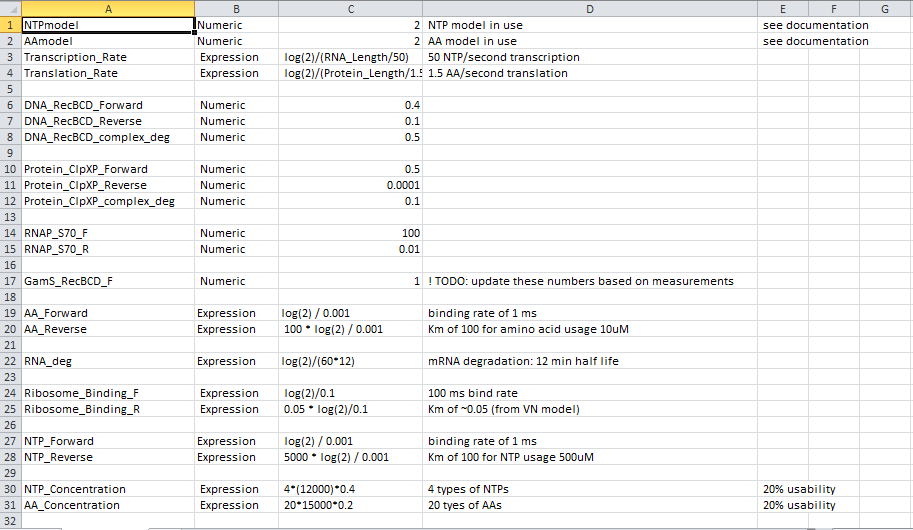
\includegraphics[width=\textwidth]{Config_E6_screenshot.png} 
		\caption{Screenshot of file 'E6\_config.csv'}
		\label{fig:reactionconfig}
		\end{center}
		\end{figure}

Figure \ref{fig:reactionconfig} shows a screenshot of the configuration file \textsf{'E6\_config.csv'}. This file is a 'Comma Separated Value' file, and is best opened in the MATLAB editor, with the 'File > Open as Text...' option. One can create custom configuration files by modifying the parameter values in this file, and saving it under a different name according to the naming convention defined above. 

		\subsection*{txtl\_component\_config (class)}	
		The txtl\_component\_config class enables users to input custom reaction parameters for the components they are using in their model. Components are found in the \textsf{components} directory in the main directory, and contain files that define proteins and promoters. The parameters present in the class and the corresponding configuration files are dependent on the components being used, but are highly analogous to the previous section. Editing of the configuration files is also carried out as above. 

	\section{List of Core Reactions}
	These reactions are currently those of Dan, and refer to the Toxin-Antitoxin System. We will modify them so that they correspond to the reactions in the TXTL toolbox. 
	
	
	\subsection{Basic}

\begin{align}
& \mathrm{RNAP} + \sigma^{70} \rightleftharpoons \mathrm{RNAP^{70}} \\
& \mathrm{RNAP} \rightarrow \phi \\
& \mathrm{RNAP^{70}} \rightarrow \sigma^{70} \\
& \mathrm{ATP} \rightarrow \mathrm{ADP} \\
& \mathrm{RecBCD} + \mathrm{GamS} \rightleftharpoons \mathrm{RecBCD}\!:\!\mathrm{GamS} 
\end{align}
	
	\subsection{Transcription}

\begin{align}
& \mathrm{DNA} + \mathrm{RNAP^{70}} \rightleftharpoons \mathrm{RNAP^{70}}\!:\!\mathrm{DNA} \\
& \mathrm{RNAP^{70}}\!:\!\mathrm{DNA} + \mathrm{NTP} \rightleftharpoons \mathrm{NTP}\!:\!\mathrm{RNAP^{70}}\!:\!\mathrm{DNA} \\
& \mathrm{NTP}\!:\!\mathrm{RNAP^{70}}\!:\!\mathrm{DNA} \rightarrow \mathrm{DNA} +  \mathrm{RNA} + \mathrm{RNAP^{70}} 
\end{align}
Dummy reaction for NTP consumption, see previous section for rates:\\
\begin{align}
& \mathrm{NTP}\!:\!\mathrm{RNAP^{70}}\!:\!\mathrm{DNA} \rightarrow \mathrm{DNA} + \mathrm{RNAP^{70}} 
\end{align}

\subsection{Translation}

\begin{align}
& \mathrm{RNA} + \mathrm{Ribo} \rightleftharpoons \mathrm{Ribo}\!:\!\mathrm{RNA} \\
& \mathrm{Ribo}\!:\!\mathrm{RNA} + \mathrm{AA} + \mathrm{ATP} \rightleftharpoons \mathrm{AA}\!:\!\mathrm{ATP}\!:\!\mathrm{Ribo}\!:\!\mathrm{RNA} \\
& \mathrm{AA}\!:\!\mathrm{ATP}\!:\!\mathrm{Ribo}\!:\!\mathrm{RNA} \rightarrow \mathrm{RNA} +  \mathrm{protein} + \mathrm{Ribo} 
\end{align}
Dummy reaction for AA consumption, see previous section for rates:\\
\begin{align}
& \mathrm{AA}\!:\!\mathrm{ATP}\!:\!\mathrm{Ribo}\!:\!\mathrm{RNA} \rightarrow \mathrm{RNA} +   \mathrm{Ribo} 
\end{align}

\subsection{Protein Degradation (if tagged)}

\begin{align}
& \mathrm{ClpX}  \rightarrow \mathrm{ClpX^*} \\
& \mathrm{protein} + \mathrm{ClpX^*} \rightleftharpoons \mathrm{protein}\!:\!\mathrm{ClpX^*} \\
& \mathrm{protein}\!:\!\mathrm{ClpX^*} + \mathrm{ATP} \rightarrow \mathrm{ClpX^*} \\
& \mathrm{ClpX^*} \rightarrow \phi
\end{align}

\subsection{Protein reactions}
\textbf{Multimerization}
\begin{align}
& \mathrm{protein} + \mathrm{protein} \rightleftharpoons \mathrm{protein\_dimer} \\
 & \mathrm{protein\_dimer} + \mathrm{protein\_dimer} \rightleftharpoons \mathrm{protein\_tetramer}
\end{align}
\textbf{Repression}\\
Here the DNA has a promoter which is repressed by protein A. For example, $tetR\_dimer$ can repress $ptet\textrm{--}rbs\textrm{--}gene$.
\begin{align}
& \mathrm{protein\_A} + \mathrm{DNA\_A} \rightleftharpoons \mathrm{DNA\_A}\!:\!\mathrm{protein\_A} 
\end{align}
Notice that in the transcription step, there is no reaction for RNA polymerase binding to the protein-bound DNA, hence repression. \\

\noindent \textbf{Maturation}\\
A few proteins, like $ClpX$ and $deGFP$, undergo maturation. 
\begin{align}
& \mathrm{protein}  \rightarrow \mathrm{protein^*}
\end{align}
\subsection{Other Degradation}

\begin{align}
& \mathrm{DNA} + \mathrm{RecBCD} \rightleftharpoons \mathrm{DNA}\!:\!\mathrm{RecBCD} \\
& \mathrm{DNA}\!:\!\mathrm{RecBCD} \rightarrow \mathrm{RecBCD} \\
& \mathrm{RNA} + \mathrm{RNase} \rightleftharpoons \mathrm{RNA}\!:\!\mathrm{RNase} \\
& \mathrm{RNA}\!:\!\mathrm{RNase} \rightarrow \mathrm{RNase} \\
& \mathrm{Ribo}\!:\!\mathrm{RNA} + \mathrm{RNase} \rightleftharpoons \mathrm{Ribo}\!:\!\mathrm{RNA}\!:\!\mathrm{RNase} \\
& \mathrm{Ribo}\!:\!\mathrm{RNA}\!:\!\mathrm{RNase} \rightarrow \mathrm{RNase} + \mathrm{Ribo} \\
& \mathrm{AA}\!:\!\mathrm{ATP}\!:\!\mathrm{Ribo}\!:\!\mathrm{RNA} + \mathrm{RNase} \rightleftharpoons \mathrm{AA}\!:\!\mathrm{ATP}\!:\!\mathrm{Ribo}\!:\!\mathrm{RNA}\!:\!\mathrm{RNase} \\
&\mathrm{AA}\!:\!\mathrm{ATP}\!:\!\mathrm{Ribo}\!:\!\mathrm{RNA}\!:\!\mathrm{RNase} \rightarrow \mathrm{RNase} + \mathrm{AA} + \mathrm{ATP} + \mathrm{Ribo} 
\end{align}
\begin{comment}
	\section{List of Parameters}
	\begin{tabular}{|c|c|c|c|c|}
	\hline
	\textbf{Parameter} & \textbf{Description} & \textbf{Value} & \textbf{Source*} & \textbf{file} \\ \hline
	Transcription\_Rate & Rate of Transcription & $50 NTP/s$ & ? & \texttt{E6\_config.csv} \\ \hline
	Translation\_Rate & Rate of Translation & $1.5 AA/s$ & ? & \texttt{E6\_config.csv} \\ \hline
	DNA\_RecBCD\_Forward & Complex formation & $0.4 ?$ & ? & \texttt{E6\_config.csv} \\ \hline
	$\sim$ & Amount of RNAP & $100 nM$ & VN & \texttt{txtl\_extract.m} \\ \hline
	$\sim$ & Amount of $\sigma 70$ & $35 nM$ & VN & \texttt{txtl\_extract.m} \\ \hline
	$\sim$ & Amount of $\sigma 28$ & $20 nM$ & VN & \texttt{txtl\_extract.m} \\ \hline	
	$\sim$ & Amount of Ribosome & $1000 nM$ & $\sim$ & \texttt{txtl\_extract.m} \\ \hline
	$\sim$ & Amount of RecBCD & $100 nM$ & Amount to match RNAP & \texttt{txtl\_extract.m} \\ \hline
		$\sim$ & Amount of NTP & $100 nM$ & Amount to match RNAP & \texttt{txtl\_extract.m} \\ \hline
	\end{tabular}
	{\scriptsize * VN refers to publications by Vincent Noireaux (U. Minnesota).}
\end{comment}

        \section{Importing Data From Plate Readers}
        Importing time series data from experiments to matlab as data structure is possible with the help of the TXTL toolbox. Currently only Biotek Plate Reader format is supported. The following steps are necessary to get get a populated data structure:
        \begin{itemize}
                \item Export your time-series data into the standard one page excel file (default export option in the Biotek plate reader sotfware).
                \item Save your excel file as a csv file (it is \textit{strongly} recommended to change the excel default delimiter to something else, e.g. ';'. We recommend Libre Office to do this conversion)
                \item After running \textit{txtl\_init}, the \textit{wholeExpfileReader} function becomes available in the path.
                \item The function \textit{wholeExpfileReader} takes the csv file path and the delimiter of the CSV file. The location of the negative control well can be given as the third optional argument.
        \end{itemize}
        This example shows how to import and the plot relevant information from the data structure.
        \lstinputlisting[lastline=33]{../examples/import_plate_reader_data.m}
\end{document}
